\documentclass[letterpaper, 10pt]{article}
\usepackage[top = 3cm, bottom = 3cm, left = 2.5cm, right = 2.5cm]{geometry}


\title{Simulation of partially clonal diploid populations with simuPOP v.1.0.8}
\author{Zhian N. Kamvar}
\date{\today}
\newcommand{\tab}{\hspace*{1.5em}}
\usepackage{mathtools, setspace, lineno}
\usepackage[pdftex, dvipdfm, dvips]{graphicx}
\usepackage[utf8]{inputenc}


\begin{document}
\maketitle
\linenumbers
\setstretch{2}
\section{Methods}
\tab All simulations were performed via the python scripted, individual-based simulation program SimuPOP (v.1.0.8) under ten different rates of sexual reproduction (0\%, 0.01\%, 0.05\%, 0.1\%, 1\%, 5\%, 10\%, 20\%, 50\%, and 100\%) referring to the proportion of offspring that would be produced via sexual reproduction. 
Each simulation consisted of a heterothallic, isolated population that contained a fixed census size of 10,000 individuals with 10 loci that had 6 to 10 alleles at each locus with variable frequencies. 

To avoid stochastic variation among rates of sexual reproduction, 100 unique seed populations were initialized with the parameters listed above.
Diploid individuals were assigned genotypes at all loci and then underwent a `burn in' period of random mating for 1,000 generations to bring the population to equilibrium. 
For each level of sexual reproduction, the seed populations were run under the specified mating scheme for 10,000 generations with a mutation rate of $1E^{-5}$ applied before mating. 
Cloned individuals were simply copied from the $F1$ to the $F2$ generation, whereas individuals derived from sexual reproduction were produced from two parents. Both operations were performed using random sampling with replacement from the $F1$ generation.
Populations were saved after every 1,000 generations and 10 sub samples of four sizes (10, 25, 50, and 100 individuals) were randomly drawn and saved in FSTAT format. 

Statistical analysis was performed using the R package \textit{poppr} (v.1.0.0). 
The summary statistics $I_A$ and $\bar{r}_d$ were calculated and their respective p-values were determined via permutation analysis.
Four different methods of permutation were utilized.
The first method was a method of permutation developed by Agapow and Burt in the program \textit{multilocus}.
This method would reshuffle genotypes at each locus in order to simulate the null hypothesis of unlinked loci. 
The second method was a method of permutation that would shuffle the alleles at each locus to simulate sexual reproduction within the observed population.
The third and fourth methods were parametric and non-parametric bootstrapping of alleles at each locus, or sampling with replacement. 
For the parametric method, at each locus, observed allele frequencies were calculated and then resampled at those frequencies to reconstruct the locus. 
The non-parametric method would simply resample alleles at each locus with replacement, regardless of frequency.
Both of the bootstrap methods would simulate the null hypothesis of sexual reproduction from a larger population. 

\section{Results}

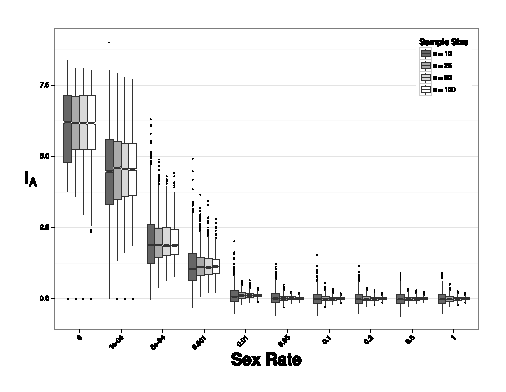
\includegraphics{figures/Ia_chart.eps}
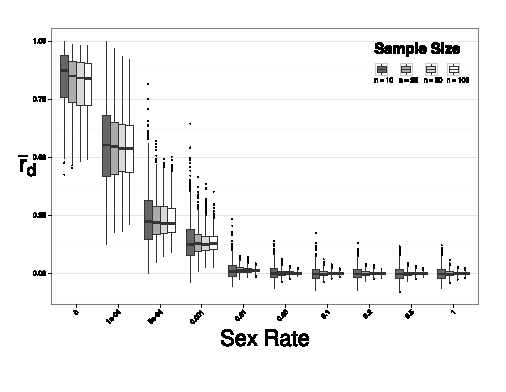
\includegraphics{figures/rbarD_chart.eps}\\
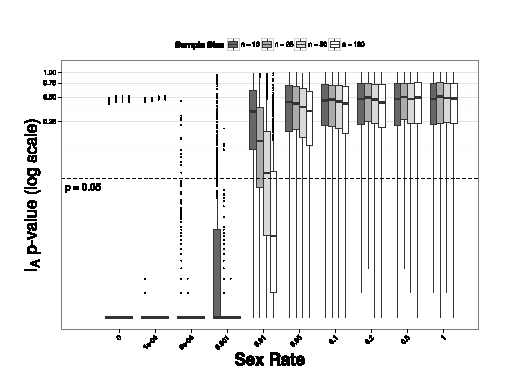
\includegraphics{figures/Ia_pval.eps}
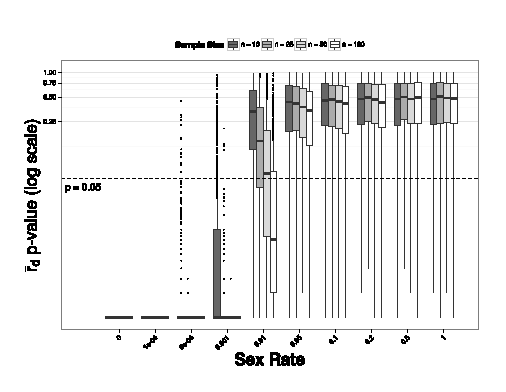
\includegraphics{figures/rbarD_pval.eps}\\

\end{document}
